\subsection{Diagramme}

\begin{tabular}{|l|l|}
	\hline
	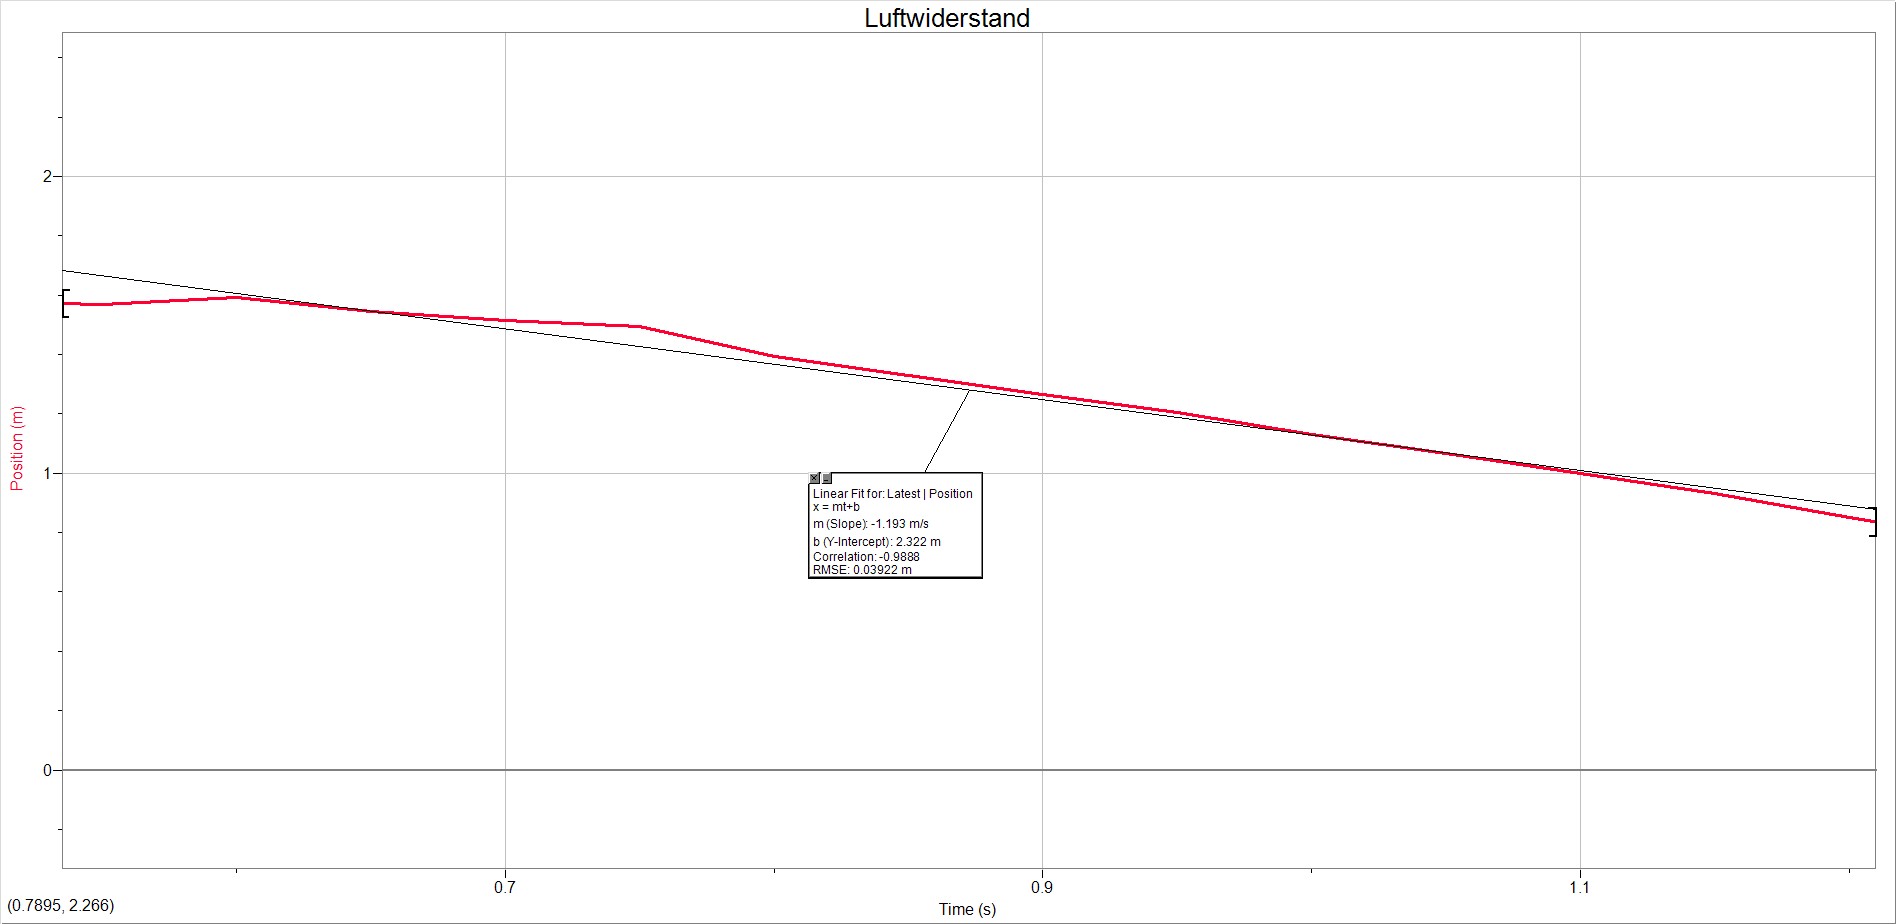
\includegraphics[width=8cm]{graphs/scr1} &
	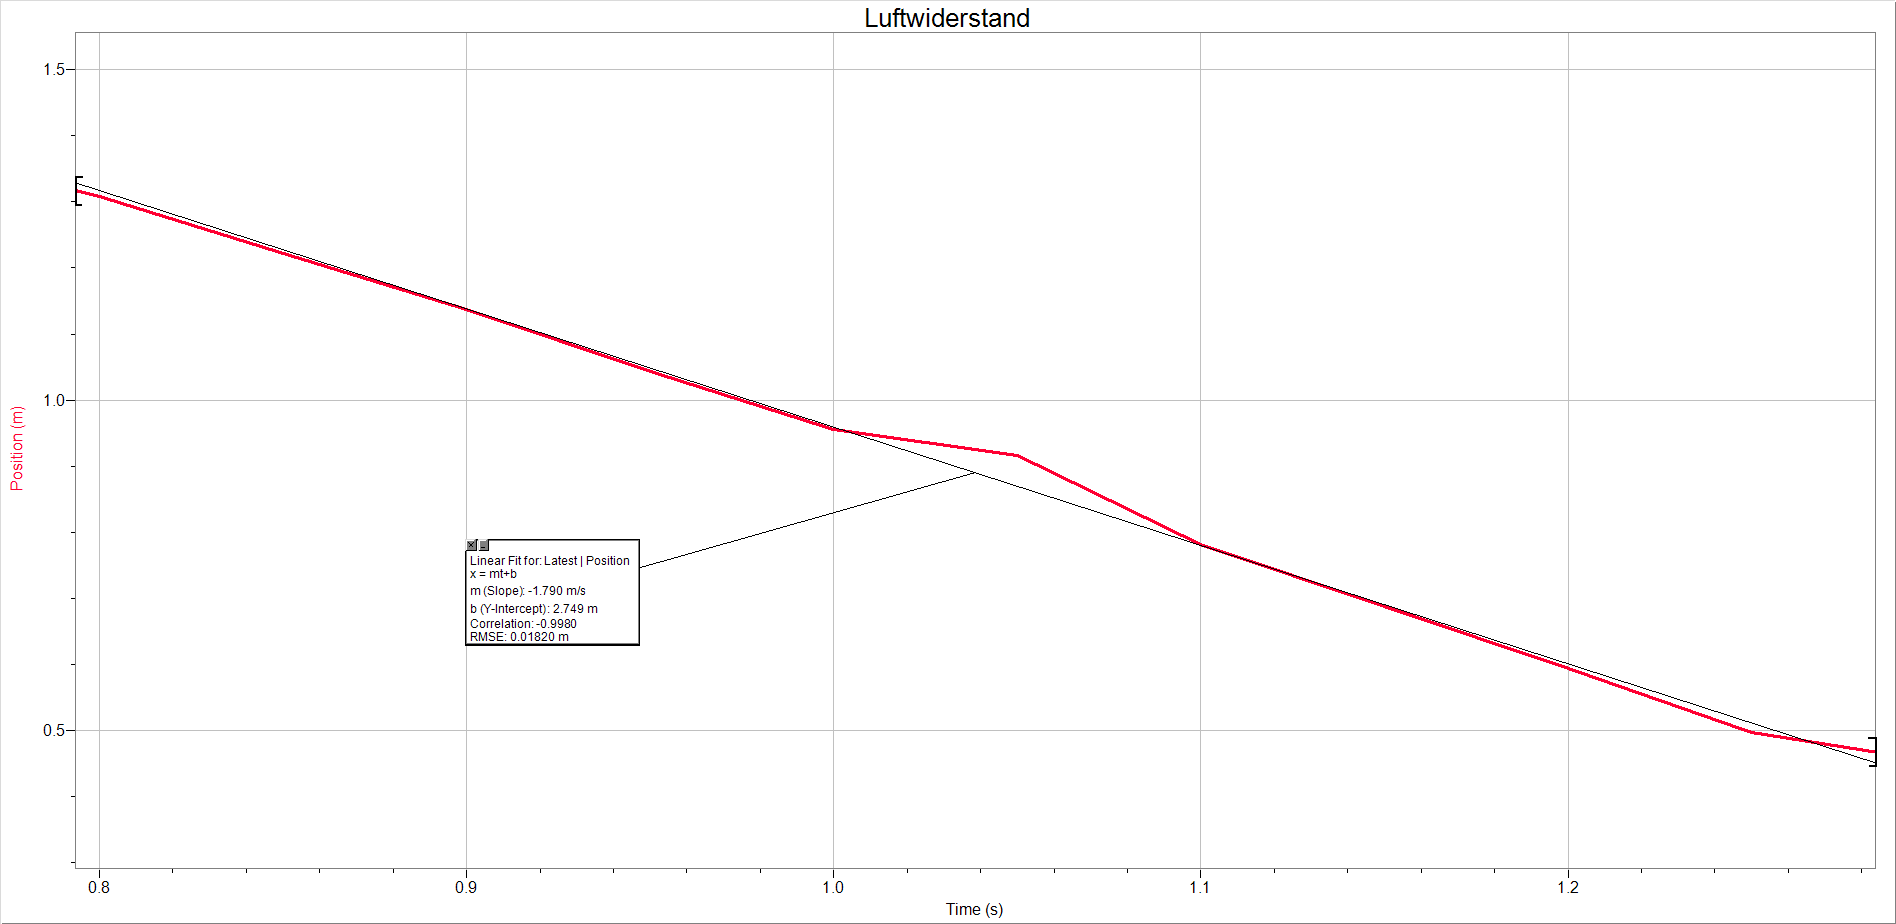
\includegraphics[width=8cm]{graphs/scr2}
	\\\hline 
	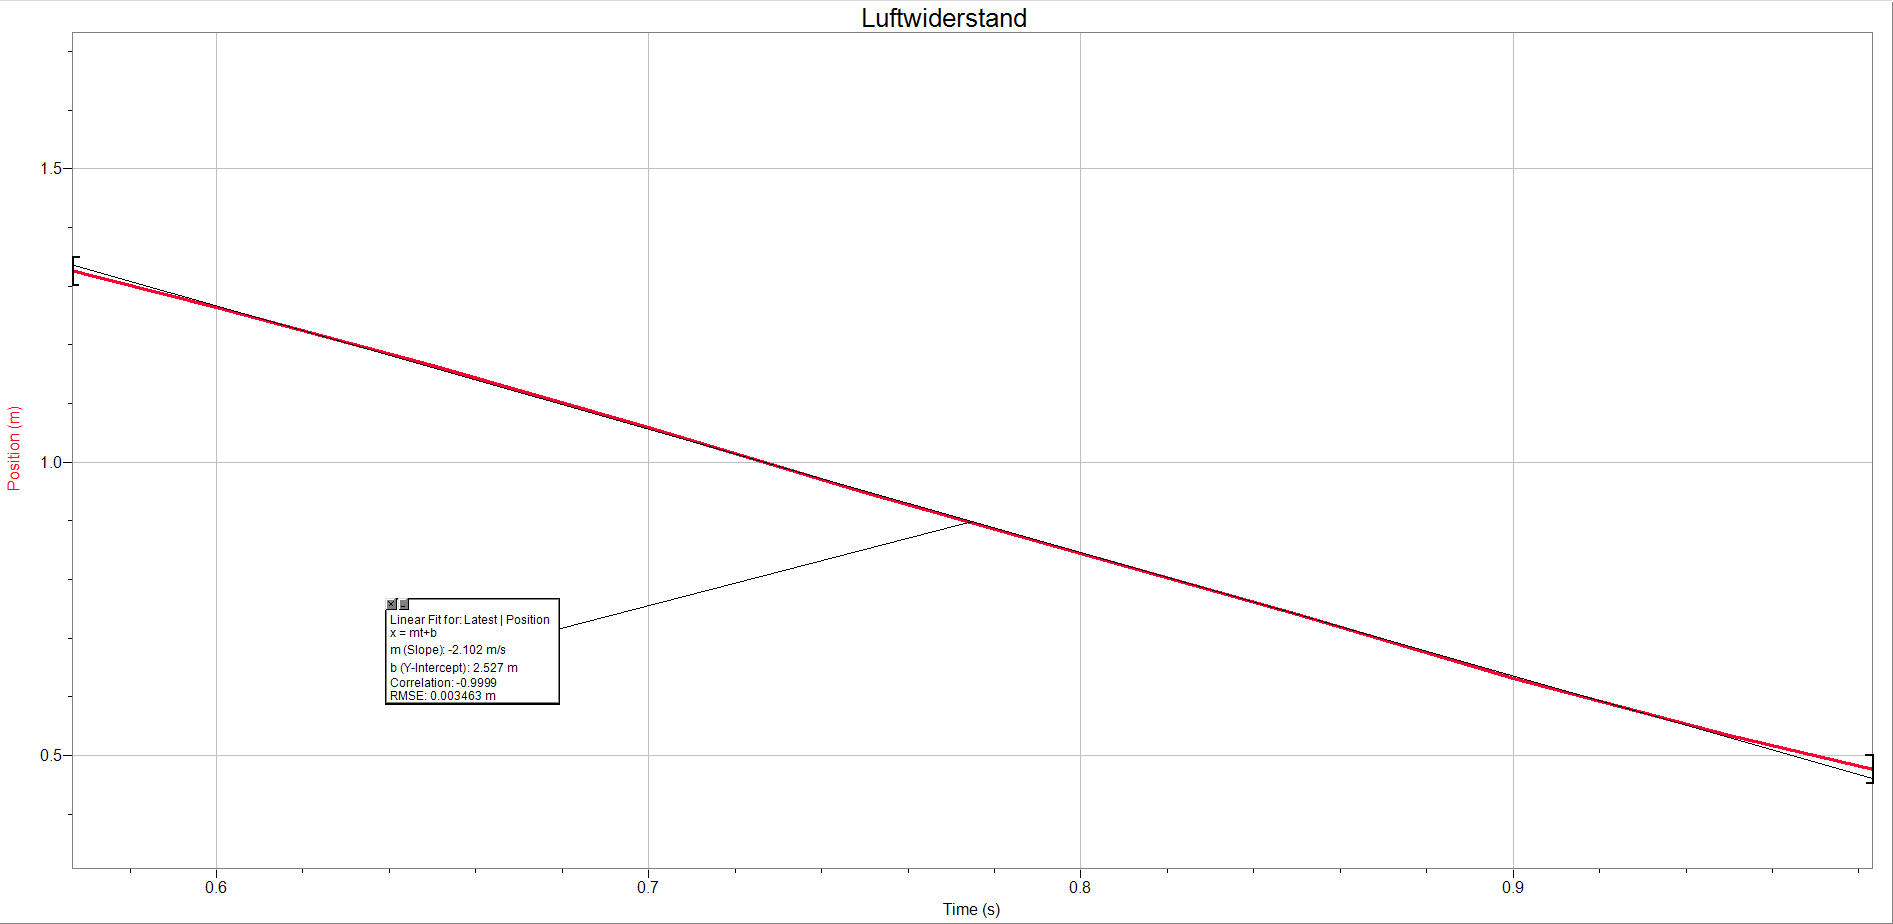
\includegraphics[width=8cm]{graphs/scr3} &
	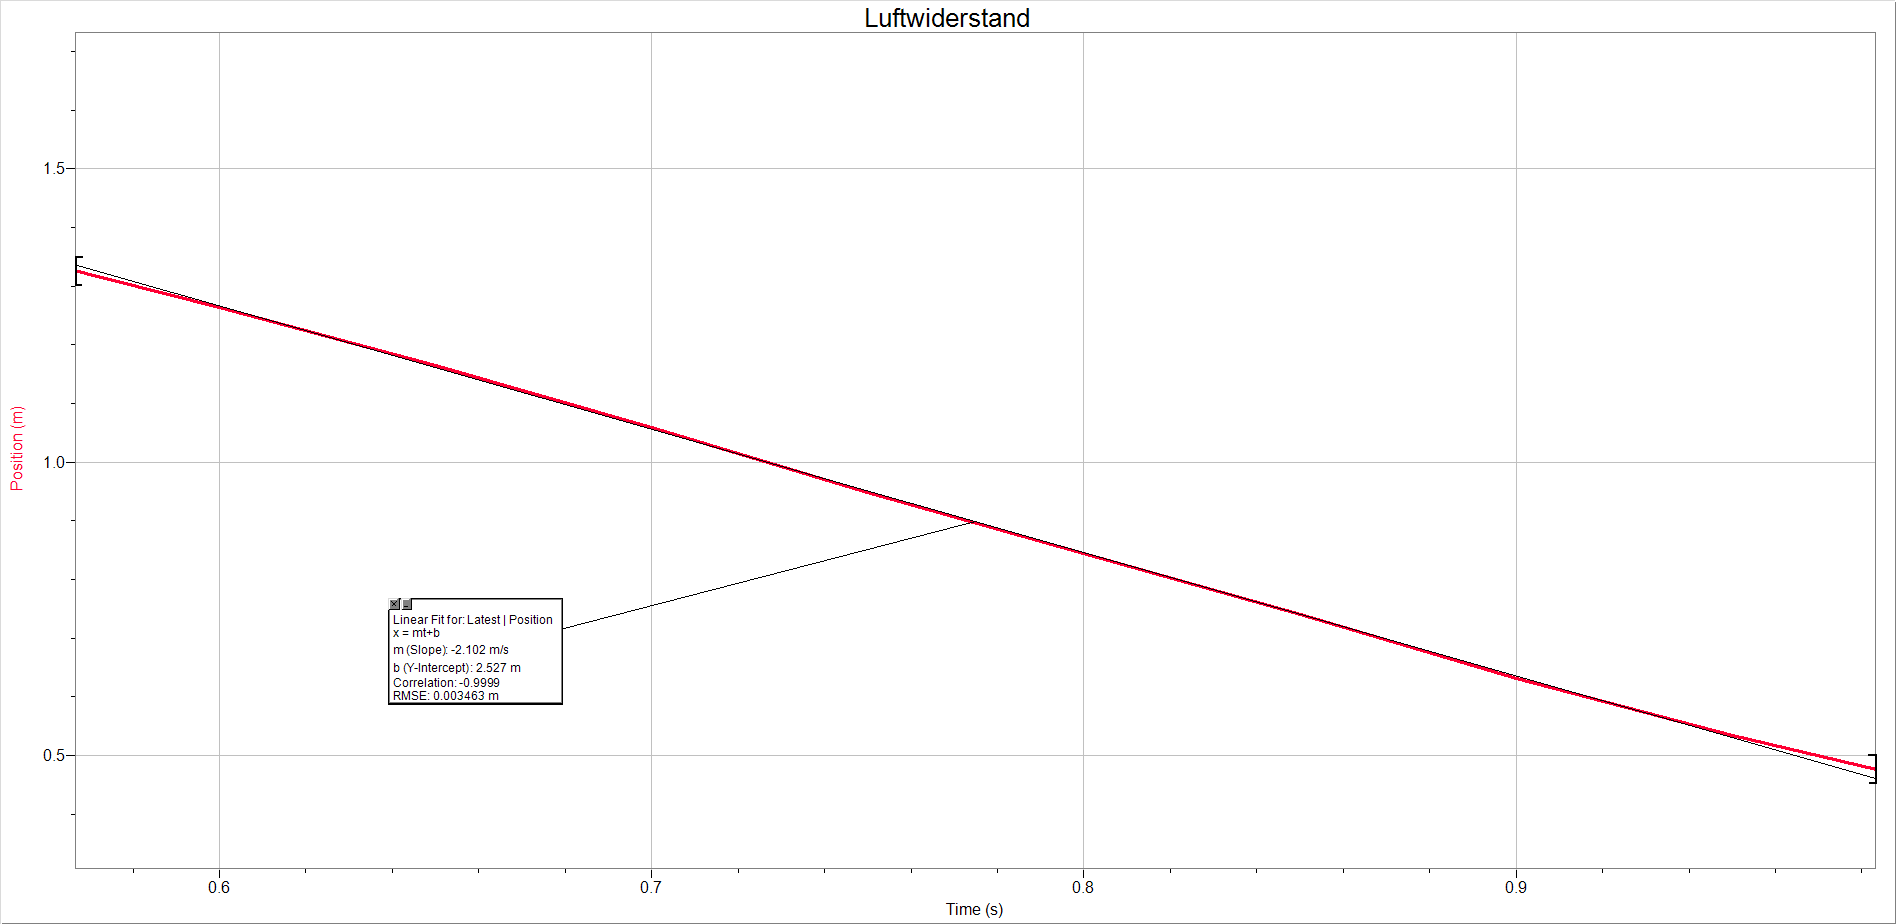
\includegraphics[width=8cm]{graphs/scr4}
	\\\hline 
	
\end{tabular}


\subsection{Auflistung Fallgeschwindigkeit}

Bei der angegebenen Geschwindigkeit handelt es sich um die \textit{Endgeschwindigkeit}

\begin{tabular}{rrr}
	\textbf{[n] Kegel} & \(v[\frac{m}{s}]\) & m[g] \\ \hline
	1 & -1.245 & 1.5 \\
	2 & -1.790 & 3 \\
	3 & -2.100 & 4.5 \\
	4 & -2.550 & 6 \\
	5 & -2.980 & 7.5 \\
\end{tabular}